\documentclass[aps,prd,superscriptaddress,nofootinbib,eqsecnum,floatfix,amsmath,longbibliography]{revtex4-2}
\usepackage[T1]{fontenc}
\usepackage{amsmath,amssymb,bm}
\usepackage{graphicx,booktabs,xcolor}
\usepackage{placeins}
\usepackage{hyperref}
\hypersetup{colorlinks=true,linkcolor=blue,citecolor=blue,urlcolor=blue}
\graphicspath{{figs/}}
\newcommand{\Tr}{\operatorname{Tr}}
\newcommand{\SU}{SU(3)}
\begin{document}
\title{Progress on SU(3) downsampling and upsampling}
\author{}
\date{October 6, 2026}
\maketitle

\section{Reference configurations and measurements}
We study factor-two reduction from a $24^4$ fine lattice to $12^4$, followed
by stochastic reconstruction of a fine field. The full pipeline is
\begin{equation}
 U\xrightarrow{S_{\bm\theta}}V\xrightarrow{B}C,
 \qquad (C,z)\xrightarrow{\mathcal L}V_0
 \xrightarrow{F_1}\widehat V\xrightarrow{F_2}\widehat U.
\end{equation}
Here $U$ denotes the complete reference fine-link configuration, with each
link in $\SU$. $S_{\bm\theta}$ is our stout-type smoothing plus $\SU$
projection, and $\bm\theta$ contains its eleven fitted coefficients.
Specifically, it mixes covariant-Laplacian polynomial, hook and local
plaquette terms, then projects the resulting matrices by polar decomposition;
it is not the standard exponential stout update. $V=S_{\bm\theta}(U)$ is
the smoothed configuration on the same fine lattice. $B$ is two-link
blocking: $C_\mu(X)=V_\mu(2X)V_\mu(2X+\hat\mu)$, where $X$ is a coarse
site and $\hat\mu$ a unit fine-lattice step. $C=B(V)$ is the coarse field.

$\mathcal L$ denotes the stochastic \emph{lift} from coarse to fine links,
before either learned flow. Its input $z$ consists of 60 independent
Haar-distributed $\SU$ detail matrices per coarse cell. Four of these,
$A_\mu$, set the first retained links; the second links are $A_\mu^\dagger
C_\mu$, and the other 56 fine links receive the remaining details.
Thus $V_0=\mathcal L(C,z)$ is a random fine field satisfying $B(V_0)=C$;
the noise is group-valued, not added to matrix entries.

$F_1$ and $F_2$ are learned invertible, gauge-equivariant field transforms.
$F_1$ produces the smeared proposal $\widehat V$ while preserving its
retained coarse products; $F_2$ produces the final fine proposal
$\widehat U$. Hats distinguish generated fields from reference fields.
Generation requires only $C,z$; the paired fine and smoothed configurations supply
training and evaluation targets. The next sections specify the smoother
and the two transforms.

\subsection{Reference ensembles}
The fine and coarse references each contain 300 configurations, generated
independently with periodic boundaries and Wilson action
\begin{equation}
 S_W[U]=\beta\sum_{x,\mu<\nu}
 \left(1-\frac13\operatorname{Re}\Tr U_{\mu\nu}(x)\right).
\end{equation}
The fine ensemble has $L=24$, $\beta=6.20$; the coarse ensemble has $L=12$,
$\beta=5.80$. Each chain starts hot, receives 1000 warmup steps, and saves
a configuration every 100 steps. A step is one heatbath hit plus four
overrelaxation hits, followed by reunitarization. Seed 1234 supplies the
first 50 configurations and seed 1235 the next 250, with a separate hot
start and warmup for each stream. QUDA uses single precision; full
$3\times3$ links are saved in NERSC IEEE32 little-endian format without
gauge fixing.

The static-potential check uses 20 spatial APE steps ($\alpha=0.5$),
Wilson loops with $r/a,t/a=1,\ldots,6$, an exponential fit over
$t/a=2,\ldots,5$, and a Cornell fit over $r/a=2,\ldots,6$.
With 1000 bootstrap samples and $r_0=0.5$ fm, it gives
$a_f=0.0722350(2175)$ fm and $a_c=0.137312(1608)$ fm
(Fig.~\ref{fig:scale}). Their ratio $a_c/a_f\simeq1.90$ is a measured
scale ratio, distinct from the geometric blocking factor 2.
Saved plaquette and APE-$W(2,2)$ series have lag-one correlations between
$-0.055$ and $0.070$ and estimated statistical inefficiency 1.
These checks concern the saved series, whose spacing is 100 update steps.

\begin{figure}[t]
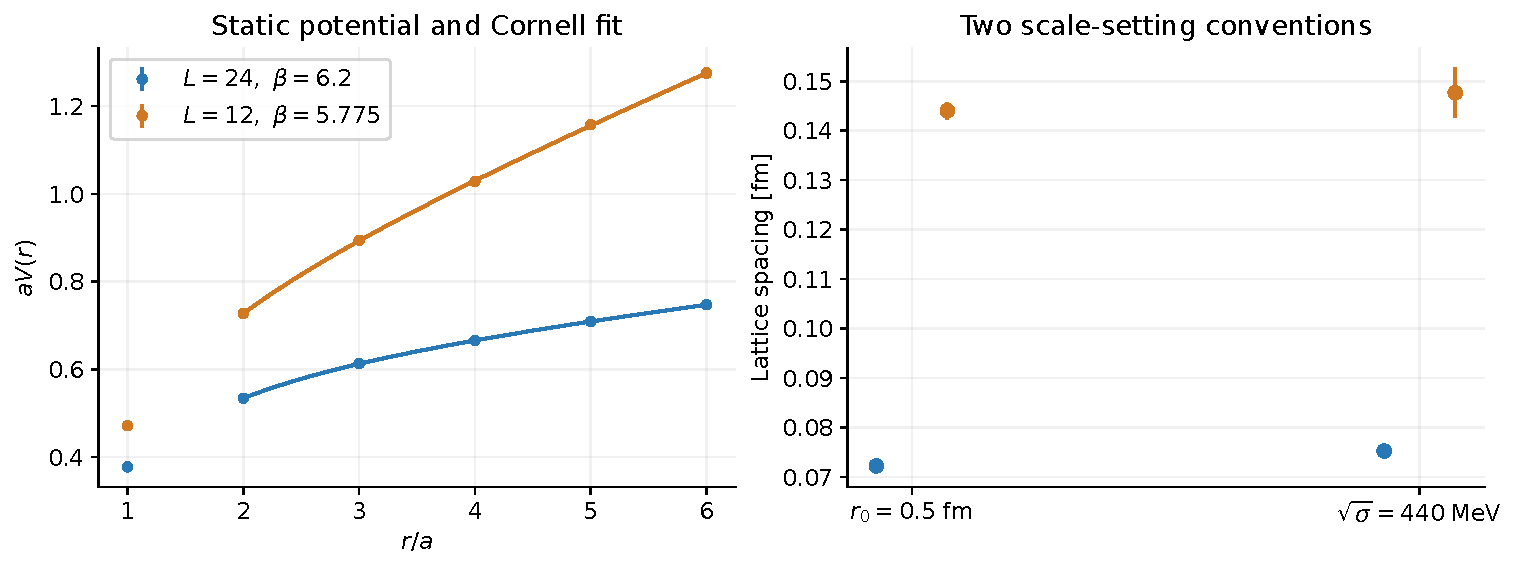
\includegraphics[width=\linewidth]{reference_scales.pdf}
\caption{Reference static potentials and lattice spacings from the Sommer
scale and string tension. The measured spacing ratio is approximately 1.90.}
\label{fig:scale}
\end{figure}

\subsection{Observables and data split}
The four observables are lattice averages of the normalized real traces
of the plaquette, $1\times2$ rectangle and $2\times2$ square, plus the
Polyakov observable. The first and third average over six unordered
planes; the rectangle averages over twelve ordered direction pairs.
For the Polyakov observable,
\begin{equation}
 O_{\rm Poly}=\frac14\sum_{\mu=0}^3|\overline P_\mu|^2,\qquad
 \overline P_\mu=\frac{1}{|\Lambda|/L_\mu}\sum_{x_\perp}
 \frac13\Tr\prod_{k=0}^{L_\mu-1}U_\mu(x_\perp+k\hat\mu).
\end{equation}
The modulus is squared \emph{after} spatial averaging of the complex trace,
then averaged over all four winding directions.

Configuration indices $i=0,\ldots,299$ are split by $i\bmod5$:
$0,1,2$ for training, 3 for validation and 4 for testing, giving
$180/60/60$. Downsampling fits 60 fixed fine training configurations,
chosen with seed 1234, against all 180 coarse training references.
Upsampling uses paired $U_i,S(U_i)$ targets; its current subset is specified
with the results below. Downsampling evaluation uses all 60 test configurations.
No test target enters a fit.

For observable $j$, let $\bar O_j,s_j$ be the output sample mean and
standard deviation, and $\bar O_{t,j},s_{t,j}$ the corresponding target
quantities. The subscript $t$ means target. With $n$ configurations,
\begin{equation}
 \bar O_j=\frac1n\sum_iO_{i,j},\qquad
 s_j^2=\frac1{n-1}\sum_i(O_{i,j}-\bar O_j)^2.
\end{equation}
The same definition applies to the target sample. These are distribution
widths; the independent-sample mean error is $s_j/\sqrt n$. We report
\begin{equation}
 \Delta_{\sigma,j}=\frac{\bar O_j-\bar O_{t,j}}{s_{t,j}},\qquad
 R_{s,j}=\frac{s_j}{s_{t,j}}.
 \label{eq:criteria}
\end{equation}
The stated distribution criterion is $|\Delta_{\sigma,j}|\le1$ and
$0.8\le R_{s,j}\le1.2$ for all four observables.

\section{Projected ``stout'' downsampling}
\subsection{Smoothing and blocking}
Here ``stout'' denotes a projected smoothing family. Unlike standard
exponential stout~\cite{morningstar}, it forms a raw transporter and
projects it onto $\SU$. Early global path mixing was replaced by the
current polynomial with hook and local-plaquette terms.

For a link-valued field $A_\mu(x)$, define the covariant transverse Laplacian
\begin{align}
 (L_UA)_\mu(x)=\sum_{\nu\ne\mu}\big[&
 U_\nu(x)A_\mu(x+\hat\nu)U_\nu^\dagger(x+\hat\mu)\nonumber\\
 &+U_\nu^\dagger(x-\hat\nu)A_\mu(x-\hat\nu)
 U_\nu(x-\hat\nu+\hat\mu)-2A_\mu(x)\big].
\end{align}
All polynomial powers use the original transporters $U$; in particular,
$L_UU$ is the six-staple sum minus $6U$. The fitted raw smoother is
\begin{align}
 W_\mu&=U_\mu+\sum_{n=1}^4(a_n+f_\mu c_n)(L_U^nU)_\mu
                  +\sum_{m=0}^2b_m(L_U^m\mathcal H)_\mu,\\
 f_\mu&=\frac16\operatorname{Re}\frac13
                   \Tr[U_\mu^\dagger(L_UU)_\mu].
\end{align}
The gauge-invariant $f_\mu$ is the mean adjacent plaquette trace minus one.
The hook field $\mathcal H$ is the unnormalized sum of twelve P5/P6 paths:
$s\mu\mu(-s)(-\mu)$ and $(-\mu)s\mu\mu(-s)$ for $s=\pm\nu$, $\nu\ne\mu$.
Thus there are eleven fitted coefficients: four $a_n$, three $b_m$ and
four $c_n$.

For the SVD $W=A\Sigma B^\dagger$, let $Q=AB^\dagger$. Smoothing and
blocking are then
\begin{equation}
 V_\mu=e^{-i\arg\det Q/3}Q,\qquad
 C_\mu(X)=V_\mu(2X)V_\mu(2X+\hat\mu).
 \label{eq:block}
\end{equation}
Only even anchors are retained. The implementation adds
$10^{-6}\operatorname{diag}(1,2,3)$ before SVD to regularize derivatives;
this fixed-colour perturbation introduces a small covariance defect.

\subsection{Fitting and results}
The initial four-coefficient polynomial was chosen by matching weak-field
Wilson propagator shapes after blocking. With left-endpoint convention
$U_\mu=1+i e^{ik\cdot x}A_\mu(k)+O(A^2)$, its kernel is
\begin{equation}
 \omega_{\mu\nu}(k)=\delta_{\mu\nu}
       +\sum_{n=1}^4a_n d_\mu(k)^{n-1}L_{\mu\nu}(k),
\end{equation}
where $d_\mu=\sum_{\rho\ne\mu}(2\cos k_\rho-2)$,
$L_{\mu\mu}=d_\mu$ and $L_{\mu\nu}=(1-e^{ik_\mu})(1-e^{-ik_\nu})$
for $\mu\ne\nu$. The rowwise powers follow because $L_UU$ has no constant
background. The propagator match sums the sixteen momenta
$k=K/2+\pi\ell$, $\ell\in\{0,1\}^4$, for each coarse momentum $K$.
Hooks and local terms are added in the subsequent ensemble fit.

The final fit starts from the polynomial-plus-hook solution, with local
coefficients zero. It minimizes four mean and four log-variance residuals:
\begin{equation}
 r_{\mu,j}=\frac{\bar O_j-\bar O_{t,j}}
 {s_{t,j}\sqrt{1/60+1/180}},\qquad
 r_{v,j}=\frac{\log[(s_j^2+10^{-12})/(s_{t,j}^2+10^{-12})]}
 {\sqrt{2/59+2/179}}.
\end{equation}
Trust-region least squares uses analytic ensemble derivatives and scaled
coordinates $12^na_n$, $12^{m+1}b_m$, $12^nc_n$ to balance polynomial
orders. Cached basis fields at retained bond positions accelerate the fit.
The objective decreases from 304.015 to 5.6853, stopping at the budget of
40 evaluations. Table~\ref{tab:coefficients} gives the frozen parameters.

\begin{table}[t]
\caption{Physical coefficients of the frozen smoother.}
\label{tab:coefficients}
\begin{tabular}{crrr}\toprule
Order & $a_n$ & $b_{n-1}$ & $c_n$\\\midrule
1 & $0.1984211682$ & $0.03923634322$ & $0.03779125486$\\
2 & $-0.02362395915$ & $0.02501181641$ & $-0.02158371669$\\
3 & $-0.002876974930$ & $0.002998340021$ & $0.002722206164$\\
4 & $-6.659929755\times10^{-5}$ & --- & $-2.232800723\times10^{-4}$\\\bottomrule
\end{tabular}
\end{table}

% BEGIN DOWNSAMPLING STATISTICS
\begin{table}[t]
\caption{Downsampling on 60 test fine and coarse configurations.}
\label{tab:down}\begin{tabular}{lrr}\toprule
Observable & $\Delta_\sigma$ & $R_s$\\\midrule
Plaquette & $0.208$ & $1.259$\\
$W_{12}$ & $0.288$ & $1.033$\\
$W_{22}$ & $0.294$ & $0.970$\\
Polyakov & $-0.101$ & $0.725$\\
\bottomrule\end{tabular}\end{table}
All four mean shifts pass Eq.~\eqref{eq:criteria}, but the plaquette and Polyakov widths fail the 20\% window (Table~\ref{tab:down}, Fig.~\ref{fig:down}).
% END DOWNSAMPLING STATISTICS

\begin{figure}[t]
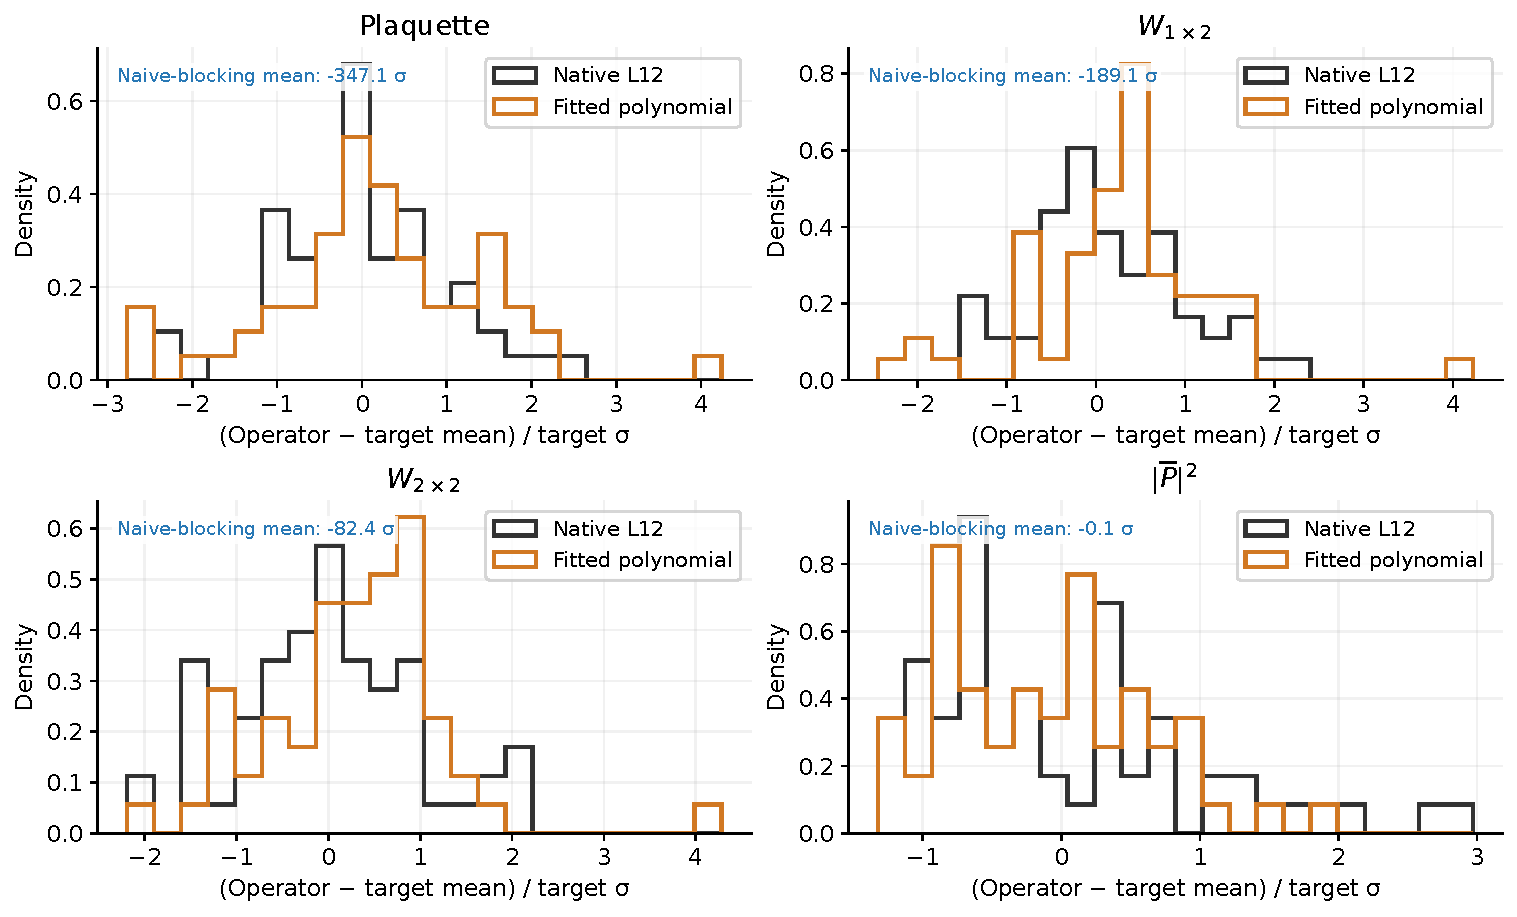
\includegraphics[width=\linewidth]{downsampling_distributions.pdf}
\caption{Downsampled and native coarse distributions on 60 test configurations,
standardized by each target mean and width.}
\label{fig:down}
\end{figure}

\section{Upsampling with Haar details and two flows}
\subsection{Coarse constraints and random details}
Each coarse cell contains $2^4$ fine sites, hence 64 fine links. Fixing four
coarse two-link products leaves 60 independent Haar $\SU$ links
(480 real detail dimensions). On retained bonds the initial lift sets
\begin{equation}
 V_{0,\mu}(2X)=A_\mu(X),\qquad
 V_{0,\mu}(2X+\hat\mu)=A_\mu(X)^\dagger C_\mu(X),
\end{equation}
with $A_\mu$ Haar, while the other 56 links are independently Haar.
This gives $B(V_0)=C$. Noise is group-valued, rather than added to link
matrices. The lift has unit Haar Jacobian and zero normalized-Haar base
log-density.

Flow~1 freezes both links on retained bonds and transforms the other
56 links, preserving $B(\widehat V)=C$. Flow~2 transforms all fine links
to learn the transport from smeared to fine fields. It does not impose
$B(S(\widehat U))=C$. This two-stage conditional construction is motivated
by cascade upscaling~\cite{cascade}.

\subsection{Local coupling and gauge equivariance}
Each sweep updates one direction and one checkerboard parity at a time.
The inactive context is
$C^{\rm ctx}=C^{(1)}+\lambda C^{(3)}$, where $C^{(d)}$ averages six staples
with transverse displacement $d$. Their lengths are three and seven links,
respectively. Odd transverse displacement puts the same-direction link on
the opposite parity, so no active link enters the context.

Following the invariant-conditioner and covariant-update principles of
Refs.~\cite{he,jin}, we use a local covariant-frame coupling rather than
the exponential Wilson-loop-derivative update of Ref.~\cite{jin}.
Its inverse and Haar Jacobian follow from the subgroup maps below,
not from that paper's coefficient bound. We construct an ordered colour frame
\begin{equation}
 H=C^{\rm ctx}(C^{\rm ctx})^\dagger=F\Lambda F^\dagger,\qquad
 \overline U=F^\dagger U,\quad
 \overline C=F^\dagger C^{\rm ctx}.
\end{equation}
Here $\Lambda$ contains the ordered eigenvalues of $H$.
In this frame, each colour pair $(i,j)$ defines a quaternion from
$M=\overline U\overline C^\dagger$:
\begin{equation}
 a=\tfrac12(M_{ii}+M_{jj}^*),\qquad
 b=\tfrac12(M_{ij}-M_{ji}^*),\qquad
 q=(a,b)/\sqrt{|a|^2+|b|^2}.
\end{equation}
A $9\to8\to6$ network uses invariant staple norms and overlaps, the
quaternion radius and site-parity bits to predict three scales and shapes.
Although the radius depends on the active link, it is unchanged by its
subgroup update; the other features depend only on inactive links or sites.
Thus the conditioner is fixed along each subgroup fibre.
Each normalized quaternion receives a radial and cubic deformation,
\begin{equation}
 \tan(\theta'/2)=e^{\eta}\tan(\theta/2),\qquad
 u\mapsto g(u)=u+\alpha u(1-u^2).
\end{equation}
Here $q_0=\cos\theta$ is the quaternion's real component and $u$ its value
after the radial step; the remaining components are rescaled to keep unit
norm. The scale $\eta$ is bounded by 2 and $|\alpha|<0.45$ makes $g$
monotone. Both are suppressed by normalized eigenvalue gaps near degeneracy;
zero or repeated-spectrum contexts use the identity update. The updated
quaternion gives an $SU(2)$ rotation $R$, applied as $FRF^\dagger U$.
The subgroup Haar Jacobians are analytic and add across couplings.

For endpoint gauge matrices $G_x,G_y$, links and contexts transform as
$U\mapsto G_xUG_y^\dagger$, $C^{\rm ctx}\mapsto G_xC^{\rm ctx}G_y^\dagger$.
The ordered frame transforms as $F\mapsto G_xFD$, where $D$ contains
arbitrary eigenvector phases. Consequently
\begin{equation}
 M\mapsto D^\dagger MD,\qquad R\mapsto D^\dagger RD,\qquad
 FRF^\dagger U\mapsto G_x(FRF^\dagger U)G_y^\dagger.
\end{equation}
The scalar conditioner and deformations commute with these phases, so they
cancel from the physical update. Composing the masked updates preserves
this equivariance. Haar details must be transformed with their fine-site
endpoints when comparing samples under a gauge transformation.

% BEGIN INVERSE STATUS
The inverse reverses the coupling order, solves the cubic with eight Newton
steps, and applies the radial map with $-\eta$. The current version keeps
fields and conditioners in double precision. Whole-flow checks gate selected
checkpoints, since deep contractions can amplify roundoff even
when each local inverse is accurate.
For the selected checkpoint, synchronized-noise $24^4$ generation gives
$9.23\times10^{-13}$ maximum gauge error and $2.83\times10^{-11}$ maximum roundtrip error. Full eight-dimensional local Haar Jacobians
agree with the analytic values to $7.33\times10^{-15}$.
The retained-product error is $1.12\times10^{-14}$; generated $\SU$ residuals are at most $5.79\times10^{-6}$ with the cached single-precision constraints.
% END INVERSE STATUS

\section{Training and current upsampling results}
% BEGIN TRAINING DESCRIPTION
The smoother is frozen and the flows have 8/2 sweeps. Adam updates all
conditioner weights, biases and long-staple weights by backpropagation.
The original fit uses 12 training and 8 validation configurations, with
conditional likelihood, smeared moments, paired transport and fine moments
trained for 4/20/3/20 epochs. Flow~1 uses
$\log q_1(V\mid B(V))=\log J_{F_1^{-1}}(V)$ on its constrained Haar details;
paired transport compares $F_2(S(U))$ with $U$.
The Adam moment loss sums covariance-weighted squared mean residuals and
squared log-variance residuals with width weight 1.

For the current calibration, Flow~1 is frozen at its stable uncalibrated
checkpoint and Flow~2 starts from a previously calibrated checkpoint.
This is not a direct continuation of the last plotted Adam checkpoint.
Calibration trains the same Flow~2 in a restricted six-parameter subspace:
for each sweep $s=1,2$, $\delta_{\eta,s}$ shifts all three raw scale
output biases, $\delta_{h,s}$ shifts all three cubic-shape output biases,
and $\delta_{\lambda,s}$ changes the long-staple weight.
Each offset is shared across sites, directions and colour pairs; other
network parameters stay fixed. The original coupling bounds and spectral
gates remain in place, preserving the equivariant construction.

The inputs are cached actual Flow~1 proposals, not reference smeared fields.
Fixed Haar draws use seed $1234+60000+i$ for configuration $i$, on
8 training and
8 validation configurations. Flow~2 changes the generated
fine configurations themselves. Its calibration score is
$\sum_j\Delta_{\sigma,j}^2+10\sum_j[\log((v_j+10^{-12})/(v_{t,j}+10^{-12}))]^2$,
where $v=s^2$. This replaces the Adam mean metric by target-width
normalization and increases the width weight to 10.
Bounded least squares uses an eight-component residual and its
finite-difference derivative with respect to six offsets (step 0.002),
with bounds $\pm1.5$ and at most 30 objective evaluations.
These derivatives are not the Haar Jacobian; no lattice backpropagation
or likelihood term is used. Finite-difference measurements are additional
to the recorded objective count. Training residuals drive the search;
selection minimizes validation score among whole-flow inverse passes with
all validation mean shifts within 2 target widths.
Six evaluations without validation improvement stop the recorded fit.
The stricter test criterion in Eq.~\eqref{eq:criteria} is unchanged.
Test configurations do not enter fitting or selection.

Adam could optimize these same offsets. The two stages differ in parameter
subspace, objective weighting and starting checkpoint, so their histories
do not establish an advantage of least squares over Adam.
The small fixed-noise fitting sample can overfit; independent test
configurations with fresh noise assess only the measured observables.
% END TRAINING DESCRIPTION

Figure~\ref{fig:up-loss} shows the recorded training and validation losses.
Each flow has one panel showing the total distribution-fitting objective
$L_{\rm total}=L_{\rm mean}+L_{\rm width}$ over the four observables.
Likelihood and paired-link warm-up losses are omitted because they have
different units. No test loss enters these curves.

\begin{figure}[t]
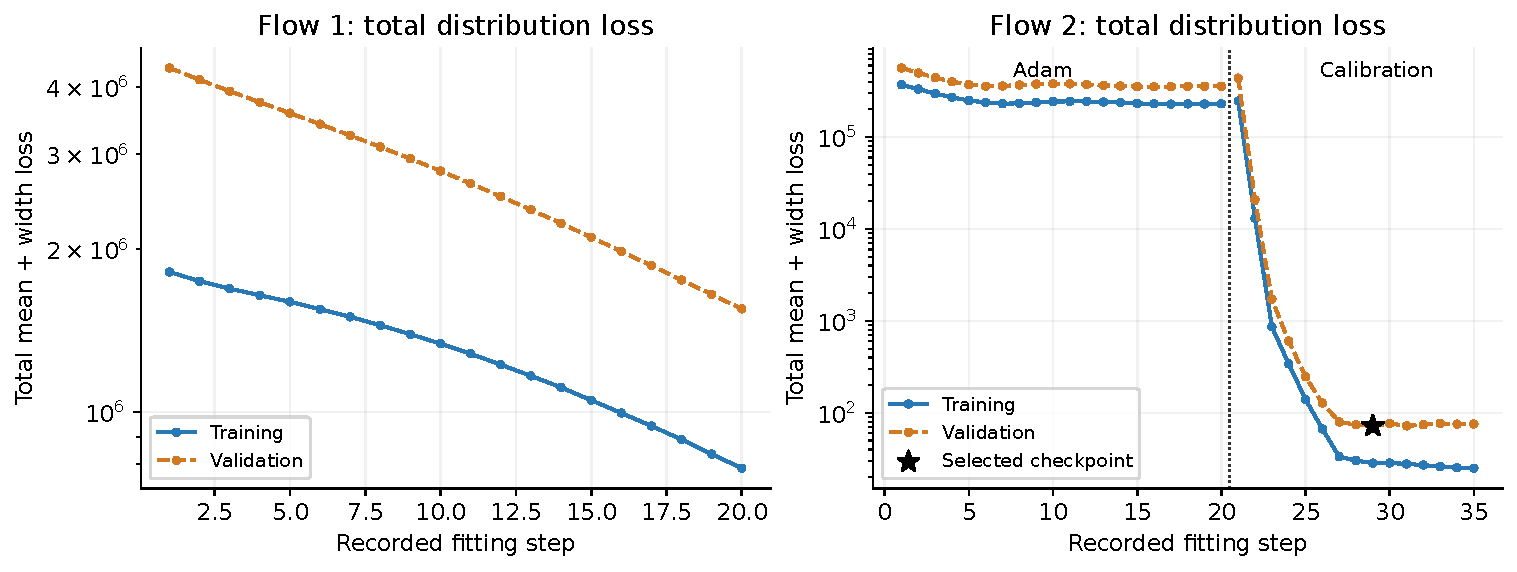
\includegraphics[width=\linewidth]{upsampling_training.pdf}
\caption{Total mean-plus-width loss for each flow. Left: 20 epochs of
Flow~1 smeared-distribution fitting. Right: 20 epochs of Flow~2 fine-distribution
fitting, followed by 15 six-offset calibration evaluations with Flow~1 frozen.
The dotted boundary separates the original covariance-weighted Adam objective
from the calibration score defined above, with its different weighting and
warm start; these segments are not joined. The star marks calibration
evaluation 9. Adam uses a pool of 12 training and 8 validation configurations
(6 training configurations per Flow~1 moment epoch); calibration uses 8 and 8.}
\label{fig:up-loss}
\end{figure}

% BEGIN EVALUATION DESCRIPTION
Evaluation uses one fresh draw for each of 60 test coarse configurations,
obtained by downsampling fine reference configurations. No rethermalization,
operator rescaling or test-target fitting is applied. Independent coarse
heatbath inputs have not been evaluated.
% END EVALUATION DESCRIPTION

For each test configuration $U_i$, the coarse input is
$C_i=B(S_{\bm\theta}(U_i))$. The Flow~1 proposal
$\widehat V_i=F_1(\mathcal L(C_i,z_i))$ is compared with the
\emph{smoothed fine-lattice reference} $V_i=S_{\bm\theta}(U_i)$,
not the original fine field or the native coarse ensemble.
The final proposal $\widehat U_i=F_2(\widehat V_i)$ is compared with
the original $U_i$. Figure~\ref{fig:up} separates these two comparisons,
using each stage's own target mean and width.
Flow~1 still fails to reproduce the smeared loop distributions. Flow~2 is
fitted to its actual generated inputs and compensates enough to bring the
four final observables roughly into overlap with their fine references.
This does not establish the full fine-field distribution or identify Flow~2
with the inverse smoother.

% BEGIN GENERATED RESULTS
\begin{table}[t]
\caption{Two-flow fine proposals on 60 test configurations.}
\label{tab:up}\small\begin{tabular}{lrrrr}\toprule
Observable & Target mean & Generated mean & $\Delta_\sigma$ & $R_s$\\\midrule
Plaquette & $0.613595$ & $0.613799$ & $1.068$ & $1.727$\\
$W_{12}$ & $0.410039$ & $0.410177$ & $0.513$ & $1.245$\\
$W_{22}$ & $0.21698$ & $0.217128$ & $0.425$ & $0.914$\\
Polyakov & $8.6875\times10^{-6}$ & $8.12545\times10^{-6}$ & $-0.130$ & $0.724$\\
\bottomrule\end{tabular}\end{table}
The final fine output fails the stated distribution criterion (Table~\ref{tab:up}, Fig.~\ref{fig:up}).
Mean shifts outside one target width: Plaquette.
Widths outside the 20\% window: Plaquette, $W_{12}$, Polyakov.
Intermediate smeared outputs fail the same criterion.
Flow~2 with teacher inputs fail the same criterion.
Flow~1 stays fixed. The fine-flow calibration used 15 objective evaluations, stopping on validation patience. Validation selects the numerically stable checkpoint.
% END GENERATED RESULTS

\clearpage
\begin{figure}[!htbp]
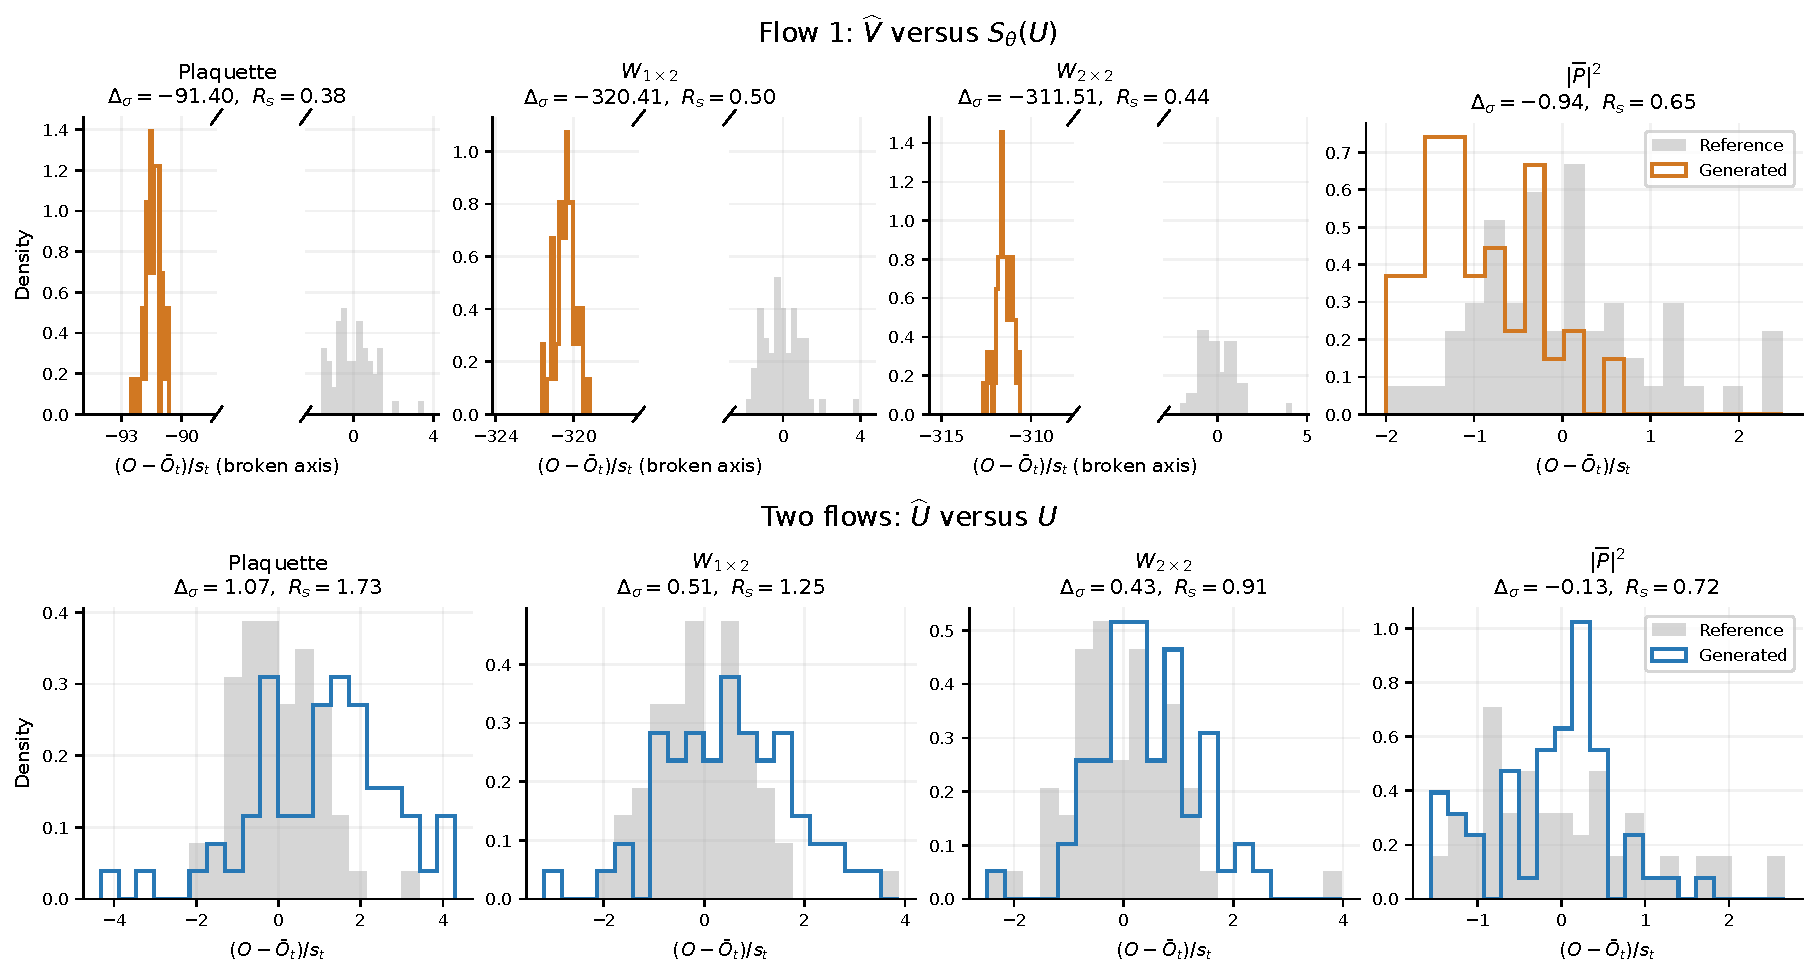
\includegraphics[width=\linewidth]{upsampling_stage_distributions.pdf}
% BEGIN UPSAMPLING CAPTION
\caption{Stage-by-stage distributions on the same 60 test configurations.
Top: Flow~1 output $\widehat V$ versus the reference fine configurations after
the frozen smoother, $S_{\bm\theta}(U)$, both on $24^4$.
Bottom: final output $\widehat U=F_2(\widehat V)$ versus original fine
references $U$. Each panel is standardized by its own reference mean and
width; annotations give $\Delta_\sigma$ and $R_s$ from Eq.~\eqref{eq:criteria}.
The top three loop panels use explicitly marked broken horizontal axes to
show the separated distributions; no samples are shifted to create overlap.}
% END UPSAMPLING CAPTION
\label{fig:up}
\end{figure}

\begin{thebibliography}{9}
\bibitem{he} J. He, X.-Y. Jin, J. C. Osborn and Y. Zhao,
``Neural Field Transformations for Hybrid Monte Carlo: Architectural Design
and Scaling,'' arXiv:2511.02018v1 (2025).
\bibitem{jin} X.-Y. Jin, ``Neural Network Gauge Field Transformation for 4D
SU(3) gauge fields,'' PoS LATTICE2023, 040 (2024), arXiv:2405.19692.
\bibitem{morningstar} C. Morningstar and M. Peardon,
``Analytic smearing of SU(3) link variables in lattice QCD,''
Phys. Rev. D \textbf{69}, 054501 (2004), arXiv:hep-lat/0311018.
\bibitem{cascade} A. Hasenfratz, E. T. Neil, L. Parato and N. Schwartz,
``Renormalization-guided cascade upscaling for lattice field generation,''
arXiv:2608.28581v1 (2026).
\end{thebibliography}
\end{document}
